\section{Methods}
The sampling rate for both algorithms is 3000HZ and the period is 333µs. Both methods will calculate the frequency value for four different frequencies. Below are the LabVIEW algorithms for calculating the value. The Goertzel-algorithms in figures ~\ref{fig:GoertzelTrue} and ~\ref{fig:GoertzFalse} correspond to steps 2 and 3 from the algorithm.
\begin{figure}[H]
  \centering
  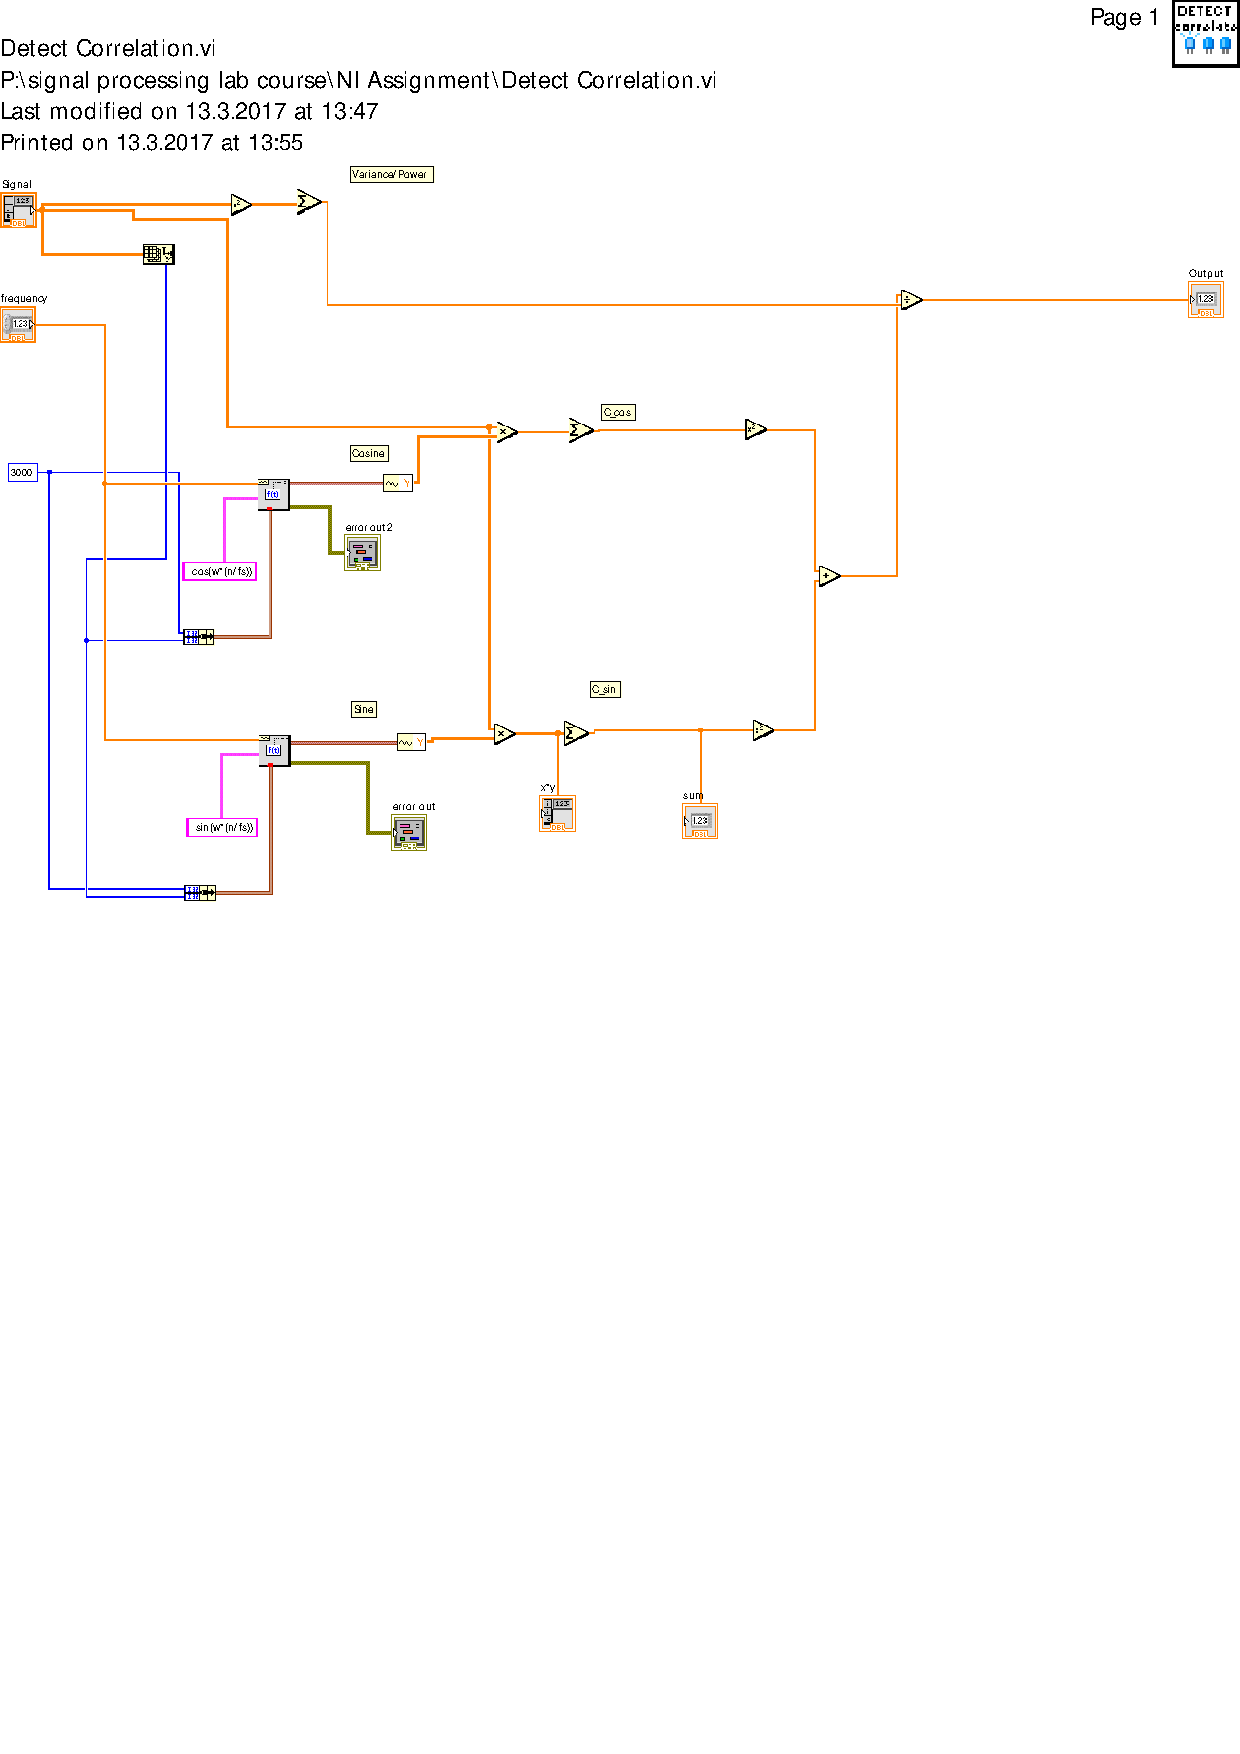
\includegraphics[width=0.8\linewidth]{detect_freq}
  \caption{LabVIEW code for Detect Correlation}
\label{fig:correlation}
\end{figure}


\begin{figure}[H]
  \centering
  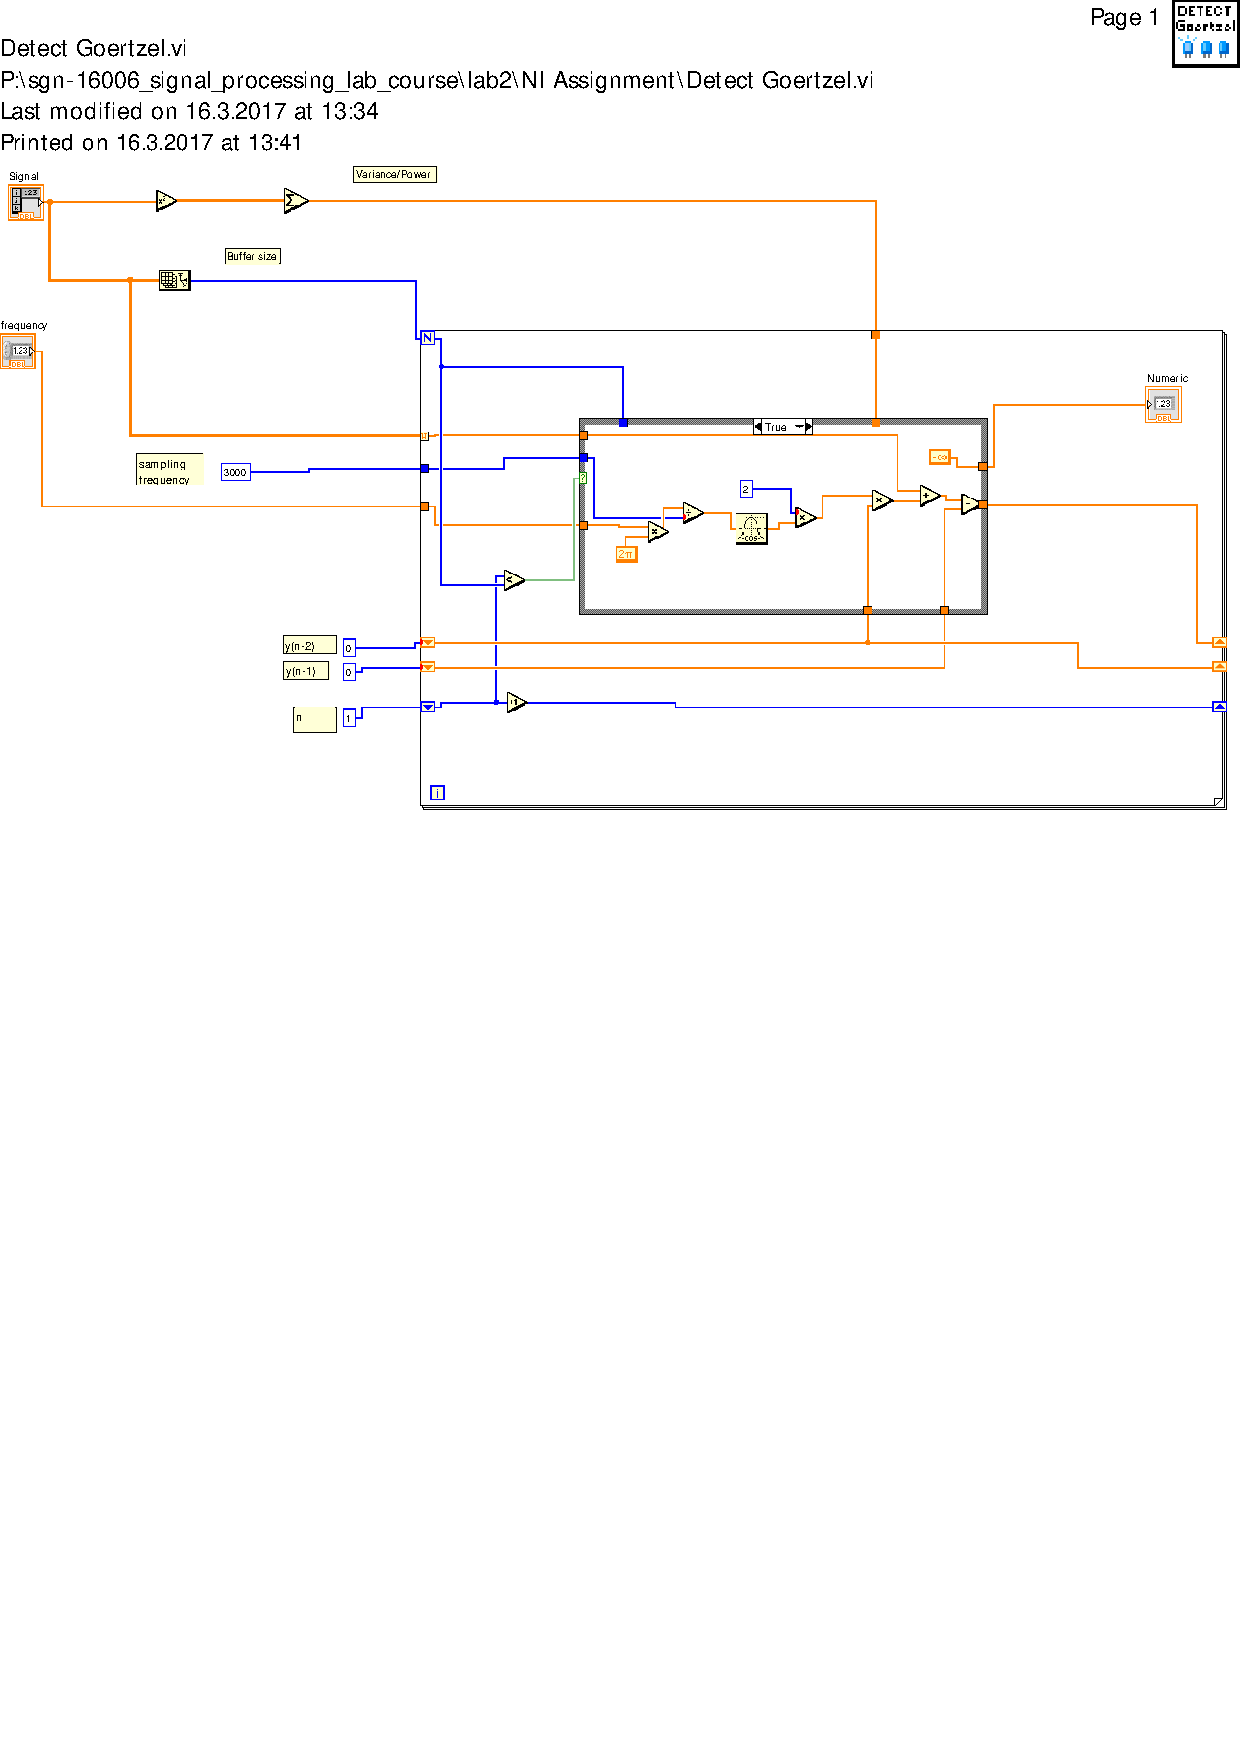
\includegraphics[width=0.8\linewidth]{detect_goertzel_true}
  \caption{Goertzel-algortihm in LabView when n $<$ N}
\label{fig:GoertzelTrue}
\end{figure}


\begin{figure}[H]
  \centering
  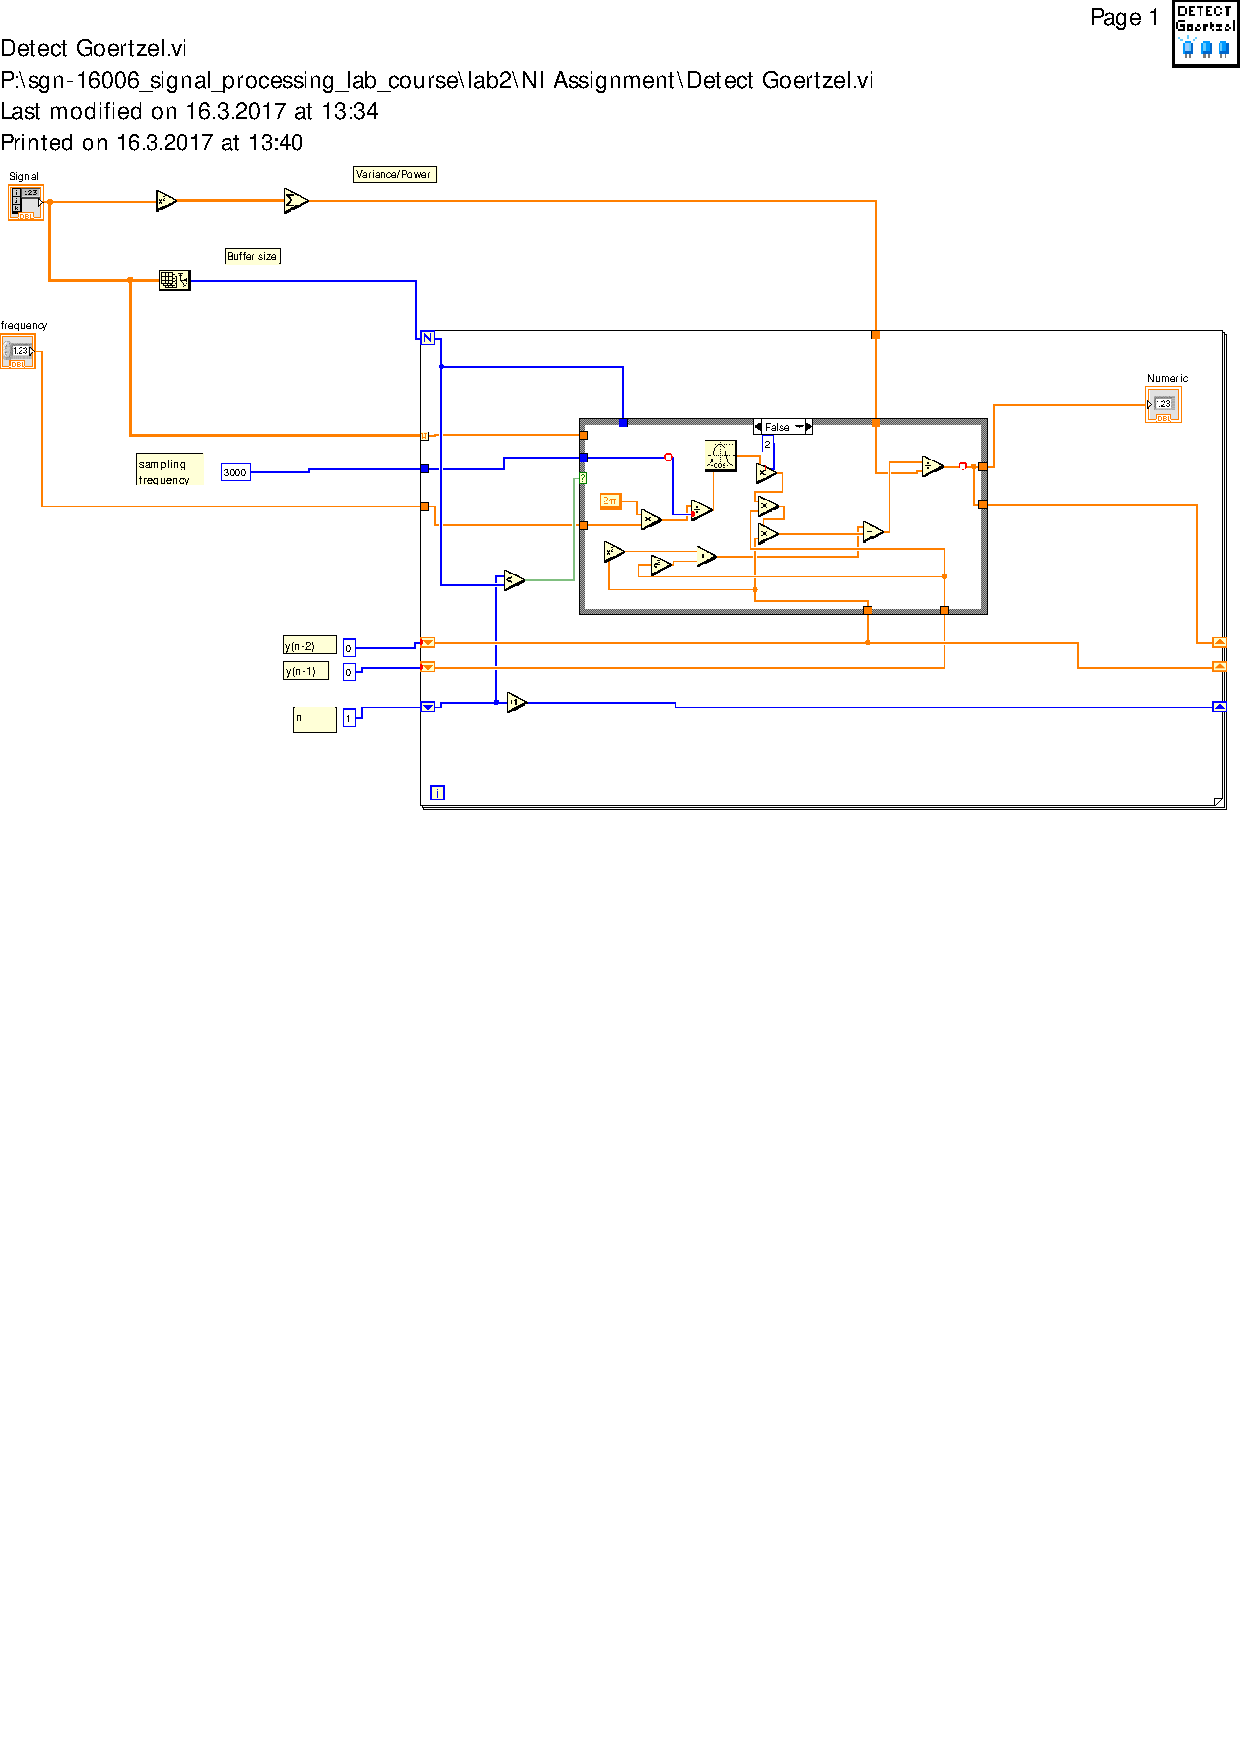
\includegraphics[width=0.8\linewidth]{detect_goertzel_false}
  \caption{Goertzel-algortihm in LabView when n = N}
\label{fig:GoertzelFalse}
\end{figure}

After the value of the frequency is calculated, we compared it to the threshold. We used the following MATLAB code to calculate the thresholds. The first part of the code goes through all the frequencies, lighting one LED at a time. The others test on one or two frequencies. We adjusted the threshold until onle the LEDs that correspond to the test signal frequency are lit. For example, second part of the Matlab code should only lit the LED that corresponds to frequency 697Hz.

\begin{lstlisting}
t = 0:1/2000:5;
x = chirp(t, 0, 5, 1000);
soundsc(x, 2000);

%%
fs = 8192;
f = 697; % This is the studied frequency
t = 0:1/fs:5;
x = sin(2*pi*t*f);
soundsc(x, fs);

%%
f = 697; % This is the studied frequency
n = 1:8192;
x = sin(2*pi*n*f / 8192);
soundsc(x);

%%
fs = 8192;
f1 = 770;
f2 = 1336;
t = 0:1/fs:5;
x = sin(2*pi*t*f1)+sin(2*pi*t*f2);
soundsc(x, fs);

%%
fs = 8192;
f1 = 852;
f2 = 1209;
t = 0:1/fs:5;
x = sin(2*pi*t*f1)+sin(2*pi*t*f2);
soundsc(x, fs);
\end{lstlisting}